\documentclass{article}

\usepackage{microtype}
\usepackage{graphicx}
\usepackage{booktabs}
\usepackage{hyperref}
\newcommand{\theHalgorithm}{\arabic{algorithm}}
\usepackage[preprint]{icml2026}
\usepackage{amsmath}
\usepackage{array}
\usepackage{multirow}
\usepackage{pgfplots}
\usepackage{xspace}
\pgfplotsset{compat=1.18}

\newcommand{\method}{BudgetFlow\xspace}
\newcommand{\trv}{TRV\xspace}
\newcommand{\taskvalue}{Task Value\xspace}
\newcommand{\tokendemand}{Estimated Token Demand\xspace}
\newcommand{\modelfit}{Model Fit\xspace}
\newcommand{\verifier}{Verifier\xspace}

\icmltitlerunning{BudgetFlow: Value-Aware Budget Governance for Agent Tasks}

\begin{document}

\twocolumn[
  \icmltitle{BudgetFlow: Value-Aware Budget Governance for Agent Tasks}

  \begin{icmlauthorlist}
    \icmlauthor{Anonymous Authors}{anon}
  \end{icmlauthorlist}

  \icmlaffiliation{anon}{Anonymous Institution, Anonymous City, Anonymous Region, Anonymous Country}
  \icmlcorrespondingauthor{Anonymous Author}{anon.email@domain.com}
  \icmlkeywords{Agent Systems, Budget Allocation, Model Routing, SWE-bench}

  \vskip 0.3in
]

\printAffiliationsAndNotice{}

\begin{abstract}
Multi-step AI agent tasks consume variable amounts of model budget, and the tasks in a batch often have unequal value. Existing model-routing work primarily decides which model should answer one request or how one task should spend its own budget. We study \emph{Batch-Level Task Budget Allocation}: a task batch shares one hard budget, and the system must allocate model opportunities across tasks before the budget is exhausted.

We introduce \method, a value-aware budget governance framework for task batches. Each task exposes four interfaces: \taskvalue, \tokendemand, \modelfit, and a \verifier. \method uses the first three signals to allocate budget and model tiers, while the \verifier settles outcomes. We evaluate \method on SWE-bench-style verified bug-fixing tasks under fixed task sets and shared hard budgets. The paper reports three primary metrics: Resolved Rate, Total Resolved Value (\trv), and \trv per Dollar.

Across one 4-policy run and three 5-policy runs over 30-task batches, \method wins the latest audited run on all three primary metrics, wins a 4-policy run on \trv and \trv per Dollar, and closely approaches the strong-model-only boundary in two runs where the strong model is unusually cost-effective. Sensitivity analyses over Task Value, budget cap, and KV-cache cost discount show how the cost-value frontier changes under different operating conditions. These results support \method as a concrete formulation of value-aware task-batch budgeting, with SWE-bench as a verified coding instantiation.
\end{abstract}

\section{Introduction}
AI agents increasingly execute multi-step tasks: they inspect context, call tools, edit artifacts, run checks, and decide whether more model calls are worth the cost. A single task can consume a few calls or dozens of calls. A batch of tasks can therefore exhaust a fixed budget before every task receives the same opportunity to succeed.

This paper studies \emph{Batch-Level Task Budget Allocation}. The setting has a task batch, one shared hard budget, model tiers with different costs and capabilities, and a \verifier that determines whether each task is resolved. The objective is to use the shared budget to produce verified task value as the central outcome.

\method is a budget governance framework for this setting. It treats each task as exposing four interfaces:

\begin{itemize}
    \item \textbf{\taskvalue}: the pre-registered value gained if the task is resolved;
    \item \textbf{\tokendemand}: the pre-run estimate of token/runway demand;
    \item \textbf{\modelfit}: evidence about how well each model tier fits the task;
    \item \textbf{\verifier}: the outcome rule that maps a completed attempt to resolved or unresolved.
\end{itemize}

The first three interfaces drive allocation decisions. The \verifier settles outcomes and defines the objective. In SWE-bench-style coding tasks, the \verifier is the test-based harness. In other domains, the same interface can be instantiated by a domain-specific outcome check.

The paper uses three primary metrics. \textbf{Resolved Rate} anchors the evaluation to standard verified success. \textbf{Total Resolved Value} (\trv) sums pre-registered \taskvalue over resolved tasks. \textbf{\trv per Dollar} measures value efficiency under the shared hard budget.

Our results are boundary-aware. \method wins the latest audited 5-policy, 30-task run on Resolved Rate, \trv, and \trv per Dollar. It wins a 4-policy run on value and value efficiency while resolving one fewer task than the strong-model-only baseline. The strong-model-only policy leads in conditions where the strong model itself forms a strong cost-value boundary. These outcomes are reported together because the scientific object is the cost-value frontier across operating conditions.

This paper makes three contributions:

\begin{enumerate}
    \item We formulate Batch-Level Task Budget Allocation with pre-registered \taskvalue, \tokendemand, \modelfit, a shared hard budget, and a \verifier-settled objective.
    \item We present \method, a task-batch budget governance framework that allocates model opportunities using value, estimated demand, model fit, and remaining budget.
    \item We evaluate \method against cheap-model-only, strong-model-only, learned task-router, and budget-only baselines, reporting Resolved Rate, \trv, \trv per Dollar, and sensitivity curves that expose operating conditions.
\end{enumerate}

\section{Problem Formulation}
\label{sec:formulation}
Let a task batch contain tasks $\mathcal{T}=\{1,\ldots,n\}$ and let $B$ denote the shared hard budget. Each task $i$ has a pre-registered value $v_i>0$, an estimated token demand $d_i>0$, and model-fit evidence $m_{i,k}$ for each model tier $k$. A policy $\pi$ chooses a sequence of actions that spend budget on model calls and task attempts. Let $c_i(\pi)$ be the spend on task $i$, and let
\[
    \sum_{i=1}^{n} c_i(\pi) \le B
\]
be the shared hard-budget constraint.

Each task has a \verifier $V_i$ that maps the final task evidence to a binary outcome:
\[
    r_i(\pi)=V_i(\pi,i)\in\{0,1\}.
\]
The primary value objective is Total Resolved Value:
\[
    \mathrm{TRV}(\pi)=\sum_{i=1}^{n} v_i\,r_i(\pi).
\]
We report three headline metrics:
\[
    \mathrm{ResolvedRate}(\pi)=\frac{1}{n}\sum_{i=1}^{n}r_i(\pi),
\]
\[
    \mathrm{TRVperDollar}(\pi)=
    \frac{\mathrm{TRV}(\pi)}{\sum_i c_i(\pi)}.
\]

The \verifier is an outcome settlement rule. The policy uses \taskvalue, \tokendemand, and \modelfit for allocation; the \verifier settles the final outcome after execution. In our SWE-bench instantiation, $V_i$ is the test-based harness. This gives a strict external success signal while preserving the task-batch allocation structure.

\begin{table*}[t]
\caption{Domain interfaces for Batch-Level Task Budget Allocation. The paper evaluates the SWE-bench instantiation.}
\label{tab:interfaces}
\centering
\small
\begin{tabular}{p{0.17\textwidth}p{0.36\textwidth}p{0.36\textwidth}}
\toprule
Interface & SWE-bench instantiation & Other task-batch instantiations \\
\midrule
\taskvalue & pre-registered criticality value & business priority, user tier, task owner value \\
\tokendemand & pre-run token/runway estimate from task metadata & expected context size, tool steps, artifact size \\
\modelfit & tier evidence from prior runs and catalog priors & domain-specific success prior by model tier \\
\verifier & test-based harness & human review, rule check, delayed business outcome \\
\bottomrule
\end{tabular}
\end{table*}

\section{BudgetFlow}
\label{sec:method}
\method maintains a shared budget ledger across the task batch. For each task, it estimates whether the next model opportunity should use the cheap model, the strong model, or defer additional spend. The policy uses three allocation inputs:

\begin{itemize}
    \item $v_i$, the \taskvalue;
    \item $d_i$, the \tokendemand;
    \item $m_{i,k}$, the \modelfit for tier $k$.
\end{itemize}

The policy also observes the remaining batch budget. Let $h$ denote budget pressure, with higher $h$ indicating less remaining headroom. Let $k_c$ be the cheap model and $k_s$ be the strong model. A simplified task-start score for giving task $i$ a strong-model opportunity is
\[
    S_i =
    \frac{v_i \cdot \max(m_{i,k_s}-m_{i,k_c},0)\cdot g(d_i)}
    {\max(\hat{c}_{i,k_s}-\hat{c}_{i,k_c},\epsilon)}
    \cdot q(h),
\]
where $\hat{c}_{i,k}$ is the estimated cost for tier $k$, $g(d_i)$ scales the opportunity by estimated runway, and $q(h)$ reduces strong-model access as the shared budget tightens. The implementation uses this score with affordability checks, learned task-router priors, and hard-budget gates. The formula captures the core allocation principle: strong-model budget is most valuable when a task has high value, sufficient expected model-fit gain, enough estimated runway, and enough remaining budget.

\method separates allocation from outcome settlement. It uses \taskvalue, \tokendemand, \modelfit, and the budget ledger to choose model opportunities. The \verifier evaluates the resulting patch or artifact after the task attempt.

\section{Experimental Setup}
\label{sec:setup}
\paragraph{Task set.}
We evaluate on fixed 30-task SWE-bench-style bug-fixing batches. Each task requires an agent to inspect a repository, edit code, and produce a patch. Outcomes are scored by the local harness and cross-checked with exported official predictions where available. Task values are pre-registered before execution.

\paragraph{Policies.}
We compare five policies:

\begin{itemize}
    \item \textbf{cheap-model-only}: every task uses the cheap model;
    \item \textbf{strong-model-only}: every task uses the strong model;
    \item \textbf{learned task-router}: chooses cheap or strong per task with a value-blind learned policy;
    \item \textbf{budget-only}: routing observes budget pressure with a value-blind policy;
    \item \textbf{\method}: value-aware task-level budget allocation.
\end{itemize}

The 4-policy run uses the four policies available in that experimental line. All mainline policies use the same task order, budget protocol, model-tier catalog, and scoring path inside a run.

\paragraph{Metrics.}
The main tables report Resolved Rate, \trv, and \trv per Dollar. Resolved Rate is written as both count and percentage. Spend is included as budget context because \trv per Dollar depends on it.

\paragraph{Sensitivity analyses.}
We report three sensitivity families on the latest audited 5-policy run. Task Value sensitivity re-scores fixed outcomes under alternate value profiles. Budget sensitivity replays the observed task order under different shared budget caps. KV Cache Cost-Discount sensitivity re-costs repeated input tokens under explicit cache-discount assumptions. These analyses use fixed observed outcomes and expose how the cost-value frontier changes under alternate accounting assumptions.

\section{Results}
\label{sec:results}
\subsection{Main Paid Evidence}
Table~\ref{tab:main-evidence} summarizes four paid task-batch runs. The latest audited 5-policy run is the strongest positive signal: \method resolves 16/30 tasks, reaches \trv 18.00, and achieves 1.81 \trv per Dollar. The next-best learned task-router resolves 15/30 tasks, reaches \trv 17.00, and achieves 1.71 \trv per Dollar.

\begin{table*}[t]
\caption{Main paid evidence. Each row reports the leader for one 30-task batch. Resolved Rate, \trv, and \trv per Dollar are the three primary metrics.}
\label{tab:main-evidence}
\centering
\small
\begin{tabular}{llcccc}
\toprule
Run & Leading policy & Resolved Rate & Spend & TRV & TRV per Dollar \\
\midrule
4-policy value-aware allocation case & \method & 14/30 (46.7\%) & \$7.52 & 18.50 & 2.46 \\
 & strong-model-only & 15/30 (50.0\%) & \$9.46 & 18.00 & 1.90 \\
\addlinespace
5-policy strong-model boundary case & strong-model-only & 17/30 (56.7\%) & \$9.95 & 20.00 & 2.01 \\
 & \method & 15/30 (50.0\%) & \$9.95 & 17.50 & 1.76 \\
\addlinespace
5-policy learned-router stress case & strong-model-only & 18/30 (60.0\%) & \$9.88 & 19.00 & 1.92 \\
 & \method & 17/30 (56.7\%) & \$9.95 & 18.50 & 1.86 \\
\addlinespace
Latest audited 5-policy positive case & \method & 16/30 (53.3\%) & \$9.95 & 18.00 & 1.81 \\
 & learned task-router & 15/30 (50.0\%) & \$9.95 & 17.00 & 1.71 \\
 & strong-model-only & 15/30 (50.0\%) & \$9.95 & 16.50 & 1.66 \\
\bottomrule
\end{tabular}
\end{table*}

The runs show three operating conditions. First, value-aware allocation can protect high-value tasks and improve \trv and \trv per Dollar even when it resolves one fewer task than strong-model-only. Second, a strong model can be the best boundary when it is both capable and cost-effective under the cap. Third, with the latest audited policy, \method improves all three primary metrics against the five-policy table.

\subsection{Full Latest 5-Policy Table}
Table~\ref{tab:latest} gives the full latest audited run. \method leads all three primary metrics. This table is the main point comparison; the next section adds sensitivity curves to show how the ordering changes under alternate operating conditions.

\begin{table}[t]
\caption{Latest audited 5-policy run over 30 tasks.}
\label{tab:latest}
\centering
\small
\begin{tabular}{lccc}
\toprule
Policy & Resolved Rate & TRV & TRV/\$ \\
\midrule
\method & 16/30 (53.3\%) & 18.00 & 1.81 \\
learned task-router & 15/30 (50.0\%) & 17.00 & 1.71 \\
strong-model-only & 15/30 (50.0\%) & 16.50 & 1.66 \\
budget-only & 12/30 (40.0\%) & 13.00 & 1.31 \\
cheap-model-only & 11/30 (36.7\%) & 12.00 & 1.21 \\
\bottomrule
\end{tabular}
\end{table}

\subsection{Task-Level Model Advantage}
The latest run contains real model-tier heterogeneity. Among tasks where both cheap and strong model rows consumed model budget, six tasks are cheap-model-favorable passes and five are strong-model-favorable passes; seven comparable tasks fail under both. This explains why all-simple policies are useful controls: the strong model often helps, but the task batch also contains tasks where cheap-model execution is the better use of budget.

\section{Sensitivity Analysis}
\label{sec:sensitivity}
\subsection{Task Value Sensitivity}
Table~\ref{tab:value-sensitivity} re-scores the latest audited run under alternate Task Value profiles. \method remains ahead of the best control under equal value, criticality value, compressed criticality, and expanded criticality. A value permutation diagnostic over 64 permutations gives \method a positive margin in all samples, with median margin +1.00 \trv.

\begin{table}[t]
\caption{Task Value sensitivity on the latest audited run.}
\label{tab:value-sensitivity}
\centering
\small
\begin{tabular}{lccc}
\toprule
Value profile & BF TRV & Control TRV & Margin \\
\midrule
equal & 16.00 & 15.00 & +1.00 \\
criticality & 18.00 & 17.00 & +1.00 \\
compressed & 17.00 & 16.00 & +1.00 \\
expanded & 20.00 & 19.00 & +1.00 \\
\bottomrule
\end{tabular}
\end{table}

\subsection{Budget Sensitivity}
Figure~\ref{fig:budget-frontier} shows budget sensitivity over the latest audited run. The curve fixes observed outcomes and replays budget accounting at different caps. It therefore describes the observed cost-value frontier for this completed run. The strong-model-only policy is strongest at some low and mid caps, while \method leads at the full cap in the paid run.

\begin{figure*}[t]
\centering
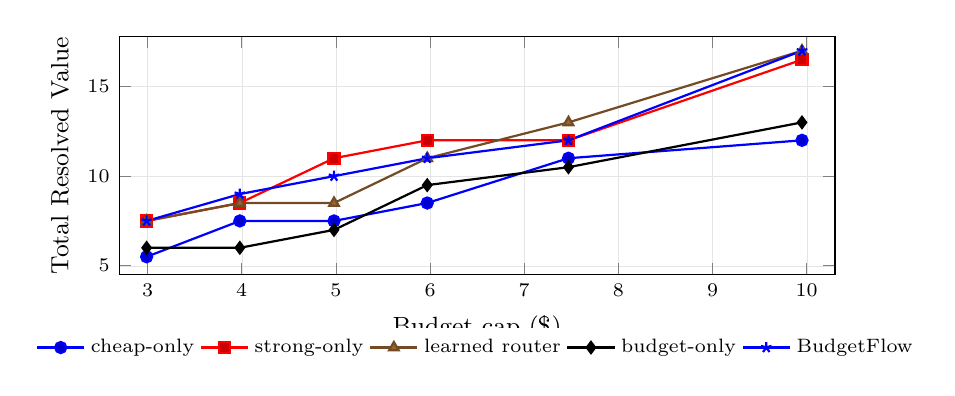
\begin{tikzpicture}
\begin{axis}[
    width=0.88\textwidth,
    height=0.38\textwidth,
    xlabel={Budget cap (\$)},
    ylabel={Total Resolved Value},
    xmin=2.7, xmax=10.3,
    ymin=4.5, ymax=17.8,
    legend style={font=\scriptsize, at={(0.5,-0.22)}, anchor=north, draw=none, fill=white, legend columns=5},
    tick label style={font=\scriptsize},
    label style={font=\small},
    grid=both,
    grid style={line width=.1pt, draw=gray!20},
]
\addplot+[mark=*, thick] coordinates {(2.99,5.50) (3.98,7.50) (4.98,7.50) (5.97,8.50) (7.47,11.00) (9.95,12.00)};
\addlegendentry{cheap-only}
\addplot+[mark=square*, thick] coordinates {(2.99,7.50) (3.98,8.50) (4.98,11.00) (5.97,12.00) (7.47,12.00) (9.95,16.50)};
\addlegendentry{strong-only}
\addplot+[mark=triangle*, thick] coordinates {(2.99,7.50) (3.98,8.50) (4.98,8.50) (5.97,11.00) (7.47,13.00) (9.95,17.00)};
\addlegendentry{learned router}
\addplot+[mark=diamond*, thick] coordinates {(2.99,6.00) (3.98,6.00) (4.98,7.00) (5.97,9.50) (7.47,10.50) (9.95,13.00)};
\addlegendentry{budget-only}
\addplot+[mark=star, thick] coordinates {(2.99,7.50) (3.98,9.00) (4.98,10.00) (5.97,11.00) (7.47,12.00) (9.95,17.00)};
\addlegendentry{BudgetFlow}
\end{axis}
\end{tikzpicture}
\caption{Budget sensitivity diagnostic on the latest audited run. Outcomes are fixed; budget accounting is replayed at alternate caps.}
\label{fig:budget-frontier}
\end{figure*}

\subsection{KV Cache Cost-Discount Sensitivity}
Table~\ref{tab:kv-sensitivity} re-costs repeated input tokens under KV-cache discounts. \method leads or is close to the best control through KV90. At KV98 and KV99 the learned task-router has the highest \trv per Dollar, while \method keeps a higher \trv than the learned task-router in the fixed-outcome table. This result is useful for serving-aware extensions: cache pricing can change the efficiency frontier while verified outcomes stay fixed.

\begin{table}[t]
\caption{KV Cache Cost-Discount sensitivity. Values are \trv per Dollar.}
\label{tab:kv-sensitivity}
\centering
\small
\begin{tabular}{lccc}
\toprule
KV profile & BF & Best control & BF margin \\
\midrule
KV0 & 1.81 & 1.71 & +0.10 \\
KV50 & 3.26 & 3.14 & +0.11 \\
KV90 & 9.06 & 8.98 & +0.09 \\
KV98 & 14.08 & 14.28 & -0.20 \\
KV99 & 15.13 & 15.41 & -0.29 \\
\bottomrule
\end{tabular}
\end{table}

\section{Related Work}
\label{sec:related}
\paragraph{Model routing and cascading.}
RouteLLM learns per-query routers from preference data~\cite{routellm}. Cascade Routing studies model routing and cascading for individual queries~\cite{cascade-routing}. RouteNLP targets enterprise query routing~\cite{routenlp}. UCCI calibrates uncertainty for cost-optimal cascade routing~\cite{ucci}. These works make model selection a first-class cost-quality problem. \method operates at the task-batch layer: many multi-step tasks share one hard budget, and the policy allocates scarce model opportunities across tasks with different values.

\paragraph{Budgeted agents.}
INTENT studies budget-constrained tool use inside a single agent task~\cite{intent}. This is a complementary layer to Batch-Level Task Budget Allocation. INTENT decides how one task should spend its own tool budget; \method decides how a task batch should share one budget across tasks.

\paragraph{Cost-aware agent runtimes and coding-agent evaluation.}
OpenSquilla is a token-efficient agent runtime with model routing, diagnostics, replay, and cost-per-success framing~\cite{opensquilla}. Claw-SWE-Bench studies harnesses, adapters, prompts, patch extraction, leakage cleanup, and cost reporting for SWE-bench-style coding-agent evaluation~\cite{claw-swe-bench}. SWE-bench provides the verified coding-task substrate used by many agent evaluations~\cite{swebench}. These systems sharpen the evaluation requirements for agent tasks: cost, harness behavior, and outcome verification must be explicit.

\paragraph{Serving substrates.}
vLLM improves LLM serving through PagedAttention and KV-cache management~\cite{vllm}; SGLang accelerates structured language-model programs with runtime optimizations such as KV-cache reuse~\cite{sglang}; Dynamo exposes agentic inference concerns including cache locality and scheduling~\cite{dynamo}. These systems provide execution substrates. \method provides task-level value and budget signals that can inform priority, continuation, model opportunity, and cache-sticky scheduling in future serving-aware systems.

\section{Discussion and Future Work}
\label{sec:discussion}
\paragraph{Formulation-level generalization.}
The SWE-bench experiments instantiate the formulation in a verified coding domain. The formulation applies to task domains where tasks expose \taskvalue, \tokendemand, \modelfit, and a \verifier. Coding tasks use tests as the \verifier. Support tasks can use policy checks and service outcomes. Spreadsheet tasks can use cell-level checks or rule engines. Research and document-production tasks can use human review or domain checks. The calibration of each interface is domain-specific; the allocation objective and budget ledger are shared.

\paragraph{Boundary-aware reporting.}
The four paid runs show different frontier leaders. This is the intended evidence shape for Batch-Level Task Budget Allocation. A value-aware policy can improve \trv and \trv per Dollar, a strong model can define the best boundary in favorable conditions, and a learned task-router can be a strong control when value placement is less important. Reporting the frontier makes these cases visible.

\paragraph{Future work.}
First, \method can study finer-grained allocation inside tasks, including stage-aware routing, segment-level routing, and escalation. Second, \method can study continual policy learning, where completed runs update future stop/continue and allocation decisions while preserving auditability. Third, \method can become serving-aware by connecting \taskvalue, remaining budget, \tokendemand, and verified outcome history to serving substrates such as vLLM, SGLang, and Dynamo. Fourth, \method can extend from one budget owner to multi-tenant task budget governance, where multiple teams, users, or services share an agent execution substrate with distinct budgets and priorities.

\section{Conclusion}
BudgetFlow formulates Batch-Level Task Budget Allocation for multi-step agent tasks under a shared hard budget. The framework uses \taskvalue, \tokendemand, \modelfit, and a \verifier to connect budget allocation with verified outcomes. On SWE-bench-style coding tasks, \method improves all three primary metrics in the latest audited 5-policy run and exposes boundary conditions across multiple paid runs. The central result is a cost-value frontier view of task-batch budgeting: the useful question is how verified value changes under fixed resource constraints and strong controls.

\bibliographystyle{icml2026}
\bibliography{references}

\end{document}
